%%%%%%%%%%%%%%%%%%%%%%%%%%%%%%%%%%%%%%%%%%  不使用 authblk 包制作标题  %%%%%%%%%%%%%%%%%%%%%%%%%%%%%%%%%%%%%%%%%%%%%%
%-------------------------------PPT Title-------------------------------------
\title{氢化锆慢化剂的\\\rm{H}原子扩散与辐照动力学研究}
%-----------------------------------------------------------------------------

%----------------------------Author & Date------------------------------------
%\author[]{\vskip +10pt 姜\;\;骏\inst{}} %[]{} (optional, use only with lots of authors)
%% - Give the names in the same order as the appear in the paper.
%% - Use the \inst{?} command only if the authors have different
%%   affiliation.
\institute[BCC]{\inst{}%
%\institute[Gain~Strong]{\inst{}%
\vskip -15pt 北京市计算中心~材料计算团队}
%\vskip -20pt {\large 格致斯创~科技}}
\date[\today] % (optional, should be abbreviation of conference name)
{	%{\fontsize{6.2pt}{4.2pt}\selectfont{\textcolor{blue}{E-mail:~}\url{jiangjun@bcc.ac.cn}}}
\vskip 45 pt {\fontsize{8.2pt}{6.2pt}\selectfont{%清华大学\;\;物理系% 报告地点
	\vskip 5 pt \textrm{2025.04.22}}}
}

%% - Either use conference name or its abbreviation
%% - Not really information to the audience, more for people (including
%%   yourself) who are reading the slides onlin%%   yourself) who are reading the slides onlin%%   yourself) who are reading the slides onlineee
%%%%%%%%%%%%%%%%%%%%%%%%%%%%%%%%%%%%%%%%%%%%%%%%%%%%%%%%%%%%%%%%%%%%%%%%%%%%%%%%%%%%%%%%%%%%%%%%%%%%%%%%%%%%%%%%%%%%%

\subject{}
% This is only inserted into the PDF information catalog. Can be left
% out.
%\maketitle
\frame
{
%	\frametitle{\fontsize{9.5pt}{5.2pt}\selectfont{\textcolor{orange}{“高通量并发式材料计算算法与软件”年度检查}}}
\titlepage
}
%-----------------------------------------------------------------------------

%------------------------------------------------------------------------------列出全文 outline ---------------------------------------------------------------------------------
\section*{}
\frame[allowframebreaks]
{
	\frametitle{\textrm{Outline}}
%  \frametitle{\textcolor{mycolor}{\secname}}
  \tableofcontents%[current,currentsection,currentsubsection]
}
%在每个section之前列出全部Outline
%类似的在每个subsection之前列出全部Outline是\AtBeginSubsection[]
%\AtBeginSection[]
%{
%  \frame<handout:0>%[allowframebreaks]
%  {
%    \frametitle{Outline}
%%全部Outline中,本部分加亮
%    \tableofcontents[current,currentsection]
%  }
%}

%-----------------------------------------------PPT main Body------------------------------------------------------------------------------------
\small
\section{研究背景}
\begin{frame}
	\frametitle{研究背景}
	核反应堆中,中子慢化过程至关重要
	\begin{itemize}
		\item 裂变主要由低能量的热中子\textrm{(<0.1~eV,2200~m/s)}引发
		\item 裂变产生的中子初始能量较高:~平均能量约为\textrm{2~MeV}
		\item 没有慢化剂存在,快中子就很容易泄漏出堆芯\\
			链式反应无法稳定维持
	\end{itemize}
\begin{figure}[!ht]
\centering
\vspace*{-0.05in}
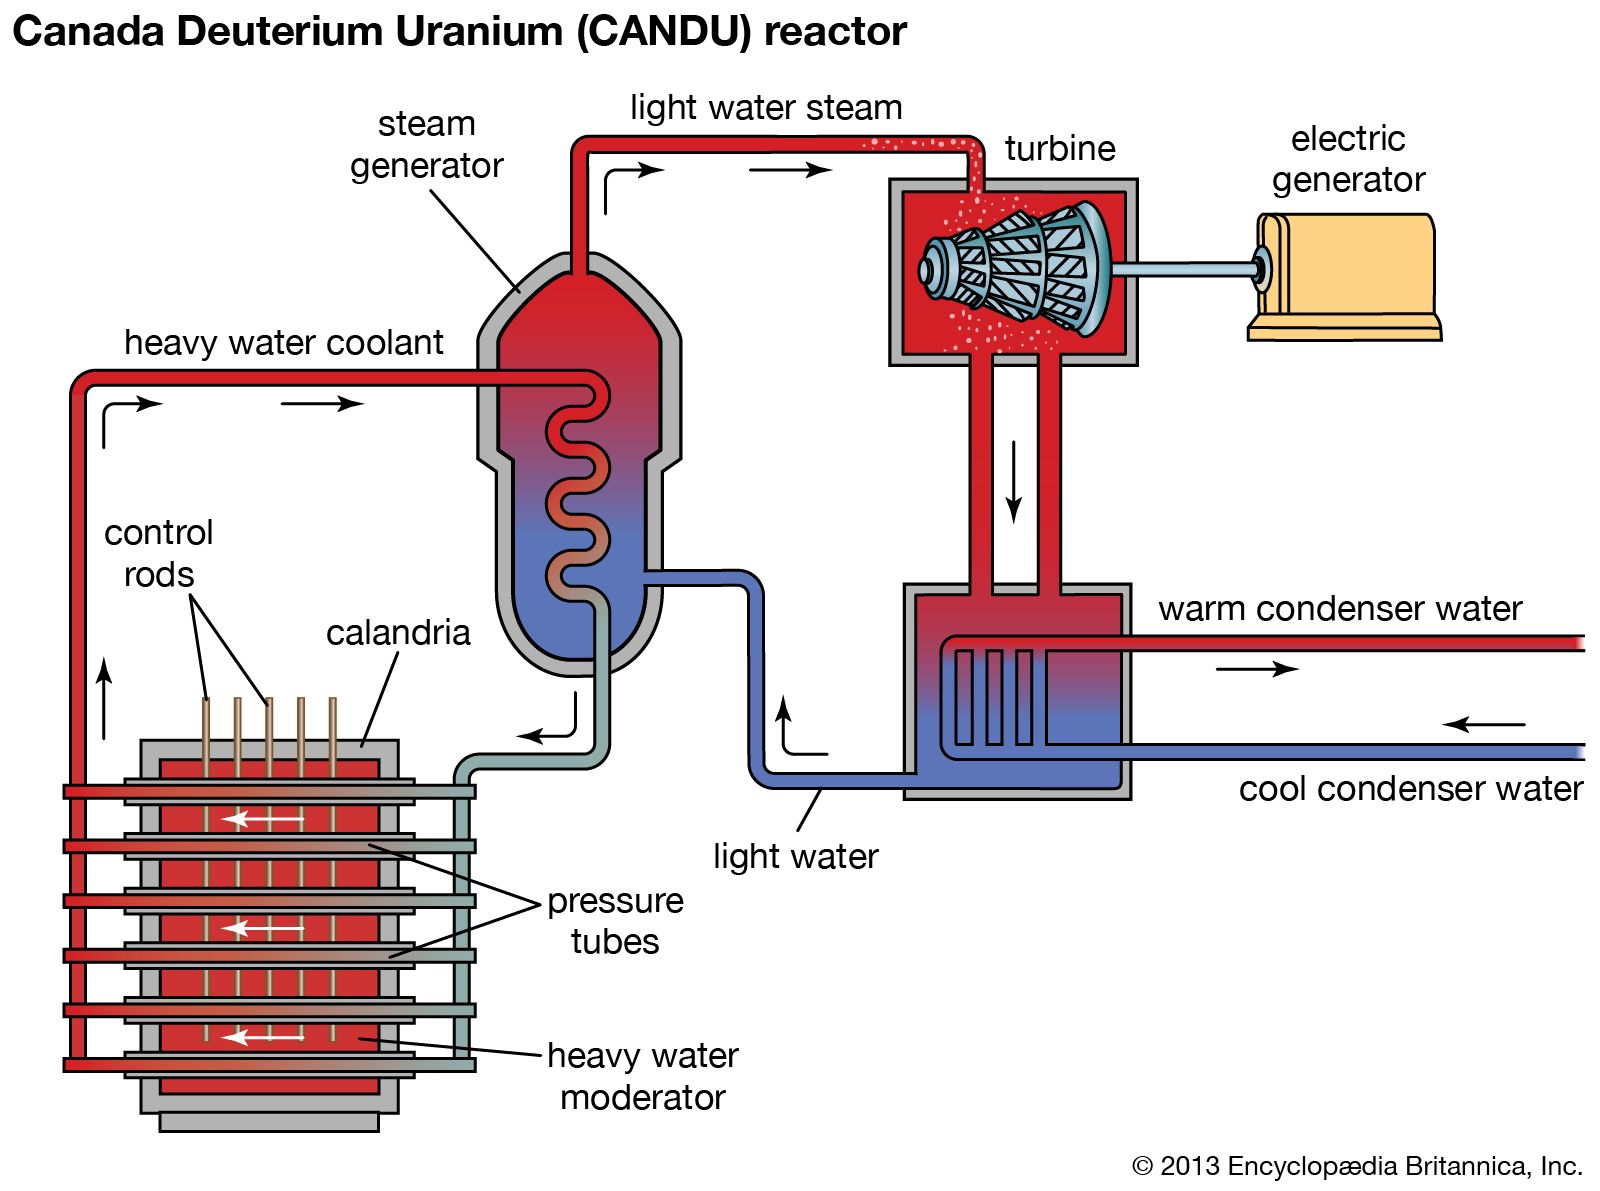
\includegraphics[height=1.20in,width=1.90in,viewport=0 0 1600 1191,clip]{Figures/Nuclear-power-plant-reactor-Canada-Deuterium.jpg}
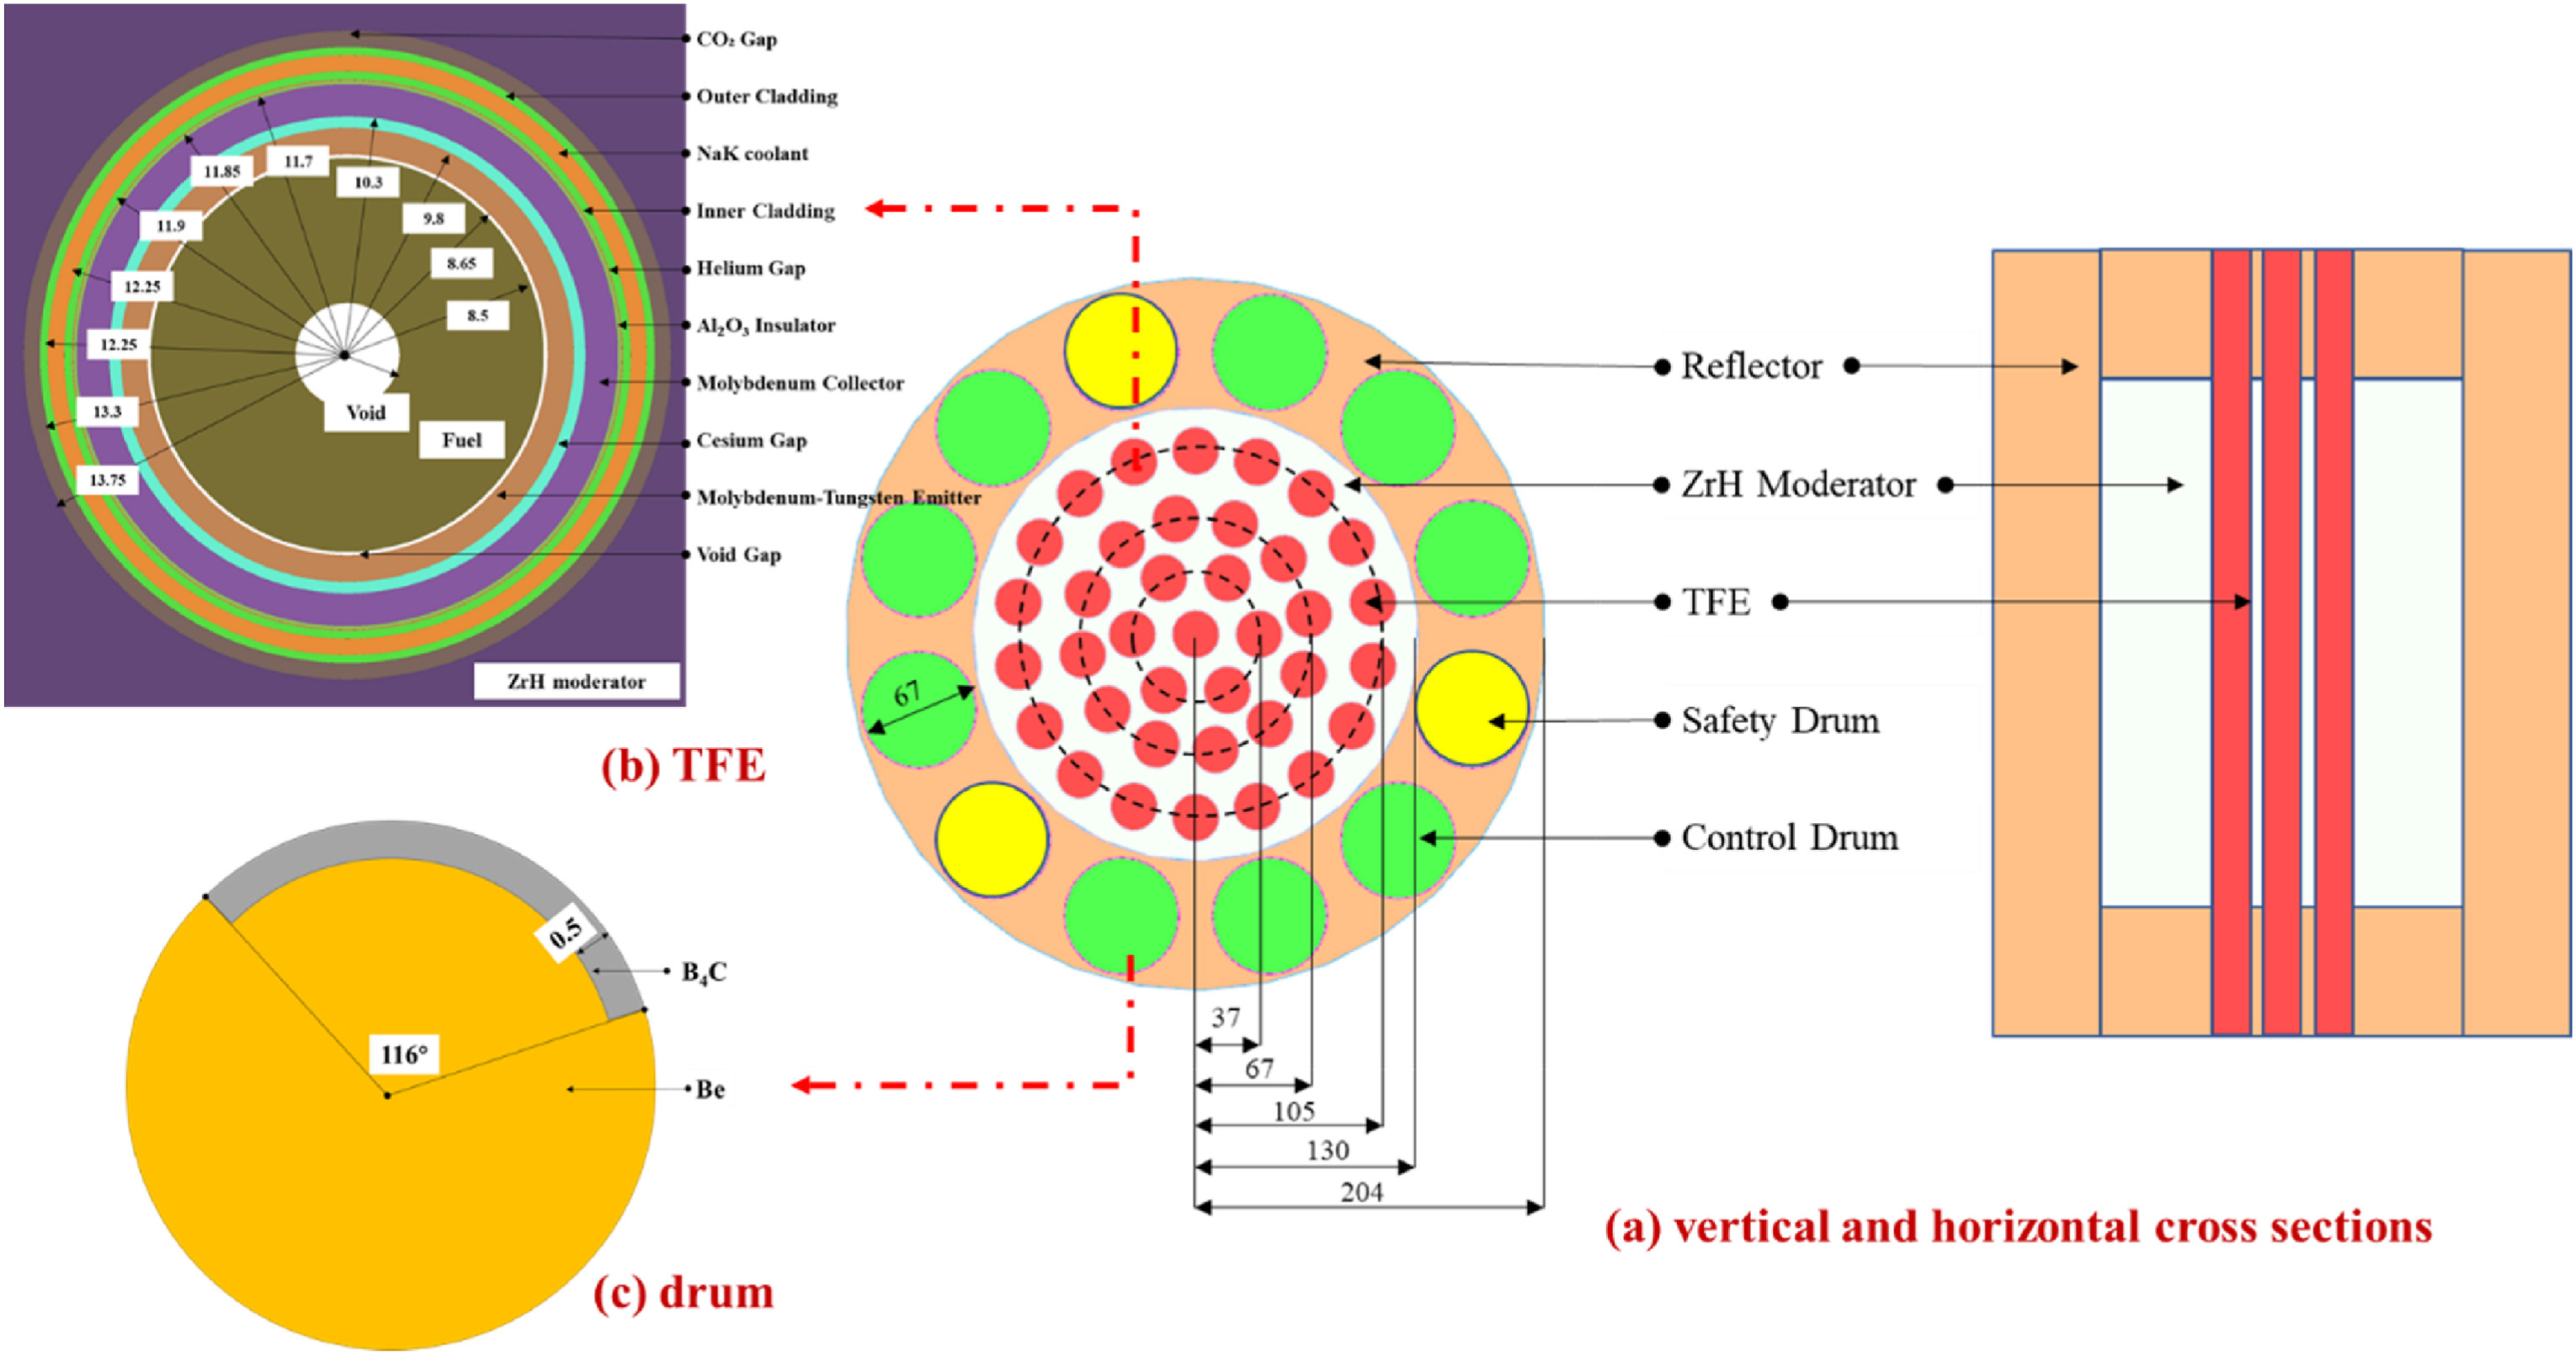
\includegraphics[height=1.00in,width=1.90in,viewport=0 0 440 230,clip]{Figures/Schematic_diagram_of_Topaz-II_reactor.jpeg}
\caption{\tiny \textrm{Schematic diagram of multi-type moderators.}}
\label{Fig:Characteristic_structures-for-the_𝛾-ZrH_𝛿-ZrH1.5_and_𝜀-ZrH2-in-Zr_hydrides}
\end{figure}
\end{frame}

\begin{frame}
	\frametitle{氢化锆结构的多样性}
金属锆对氢具有极强的亲和力,但室温下氢在锆中的固溶度却非常低\textrm{($<1\mathrm{ppm}$)},随着吸氢量的增加,会先后形成多种结构的氢-锆化合物
\begin{itemize}
	\item $\zeta$-氢化物\textrm{(\ch{Zr2H},HCP-密排六方结构)}
	\item \textcolor{blue}{$\gamma$-氢化物\textrm{(\ch{ZrH},FCT-面心四方结构)}}~\textcolor{red}{$\leftarrow$亚稳态}
	\item \textcolor{blue}{$\delta$-氢化物\textrm{(\ch{ZrH}$_{1.66}$,FCC-面心立方结构)}}~\textcolor{red}{$\leftarrow$稳态}
	\item $\varepsilon$-氢化物\textrm{(\ch{ZrH2},FCT-面心四方结构)}
\end{itemize}
\begin{figure}[!ht]
\centering
\vspace*{-0.05in}
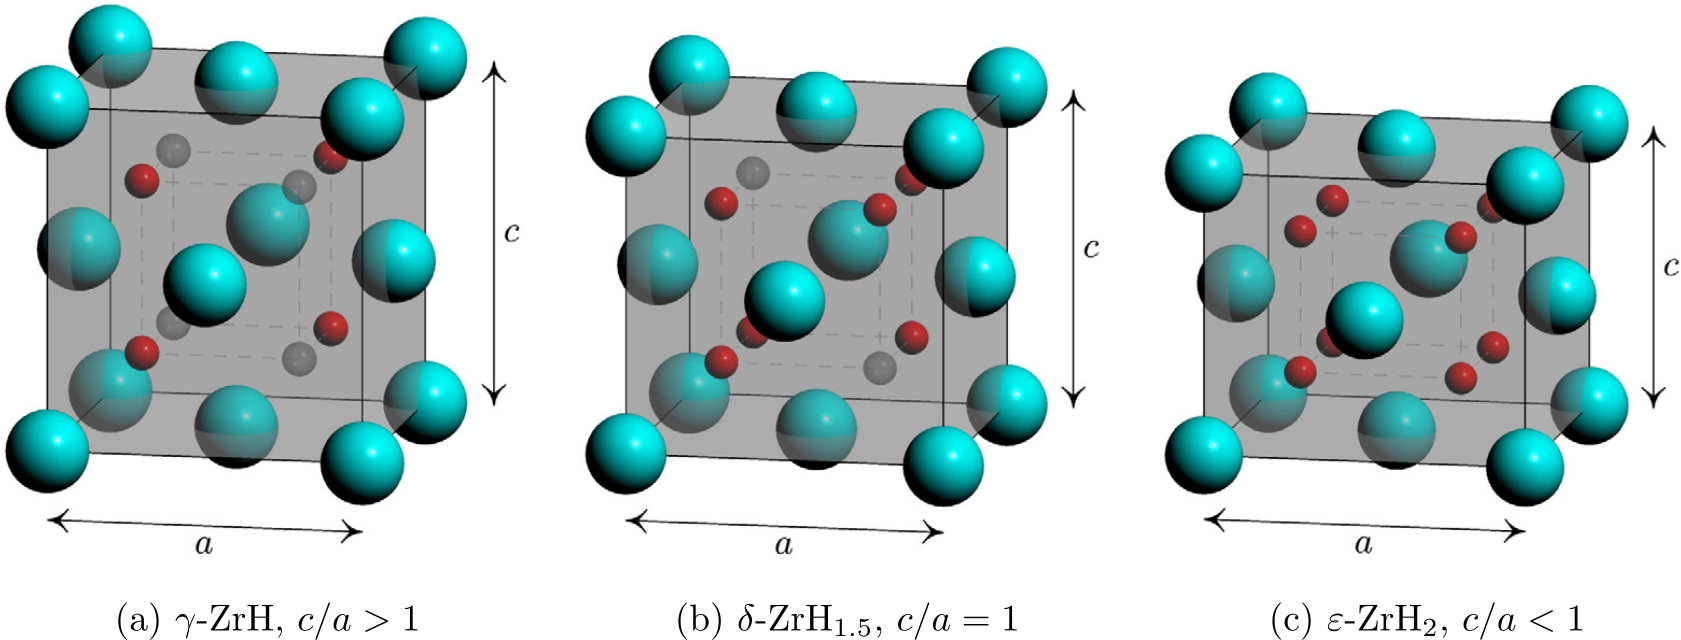
\includegraphics[height=1.50in,width=4.00in,viewport=0 0 1681 640,clip]{Figures/Characteristic_structures-for-the_ZrH_ZrH1.5_and_ZrH2-in-Zr_hydrides.png}
\caption{\tiny \textrm{Characteristic structures for the $\gamma$-ZrH, $\delta$-$\mathrm{ZrH}_{1.5}$, and $\varepsilon$-$\mathrm{ZrH}_2$ in Zr hydrides.}}
\label{Fig:Characteristic_structures-for-the_𝛾-ZrH_𝛿-ZrH1.5_and_𝜀-ZrH2-in-Zr_hydrides}
\end{figure}
%锆合金中常见的氢化物为$\gamma$氢化物和$\delta$氢化物,前者是亚稳态氢化物,后者为比较稳定的氢化物%。在没有外加应力的情况下,氢化物通常以锆基体的基面为惯习面,沿基面上的$<\mathrm{a}>$方向生长。在外加拉应力情况下,氢化锆会发生再取向,其惯习面会随着拉应力的增加逐步从基面转向\textrm{\{10-1$i$\} ($i$=1-7)}锥面,直至最后以柱面\{10-10\}为惯习面。再取向过程中,氢化物的生长方向始终沿着$<\mathrm{a}>$方向。在核燃料包壳管中,初始的氢化物都沿管子的周向分布,这与挤压管的初始织构密切相关,即锆包壳管具有基面沿管子周向分布的特征。在核反应堆服役过程中,核燃料在中子辐照下发生体积膨胀,使得包壳管被撑大,此时包壳管沿周向受到一定的拉应力,这种应力称之为环向应力\textrm{(hoop stress)}。在环向应力的作用下,当核反应堆冷却时,锆合金包壳管中的氢化物析出就会发生再取向,新的惯习面会沿着锥面或柱面。当环向拉应力超过\textrm{100~MPa}时,氢化物再取向主要会以柱面为惯习面。此时,若对比氢化物的初始分布和再取向分布,可以发现氢化物相当于转动了$90^{\circ}$,形成了大量的径向氢化物,沿锆合金包壳管厚度方向分布。这种再取向的氢化物会更容易造成锆合金包壳的失效。
\end{frame}

\section{研究目的和内容}
\begin{frame}
	\frametitle{研究目的}
	\textcolor{red}{作为慢化剂的氢化锆材料受到辐照后的微观动力学机理}:
	\vskip 2pt
	通过理论计算研究氢化锆固体中\textcolor{blue}{氢原子}在高温、密闭真空环境的扩散行为,模拟实验结果
\begin{figure}[!ht]
\centering
\vspace*{-0.05in}
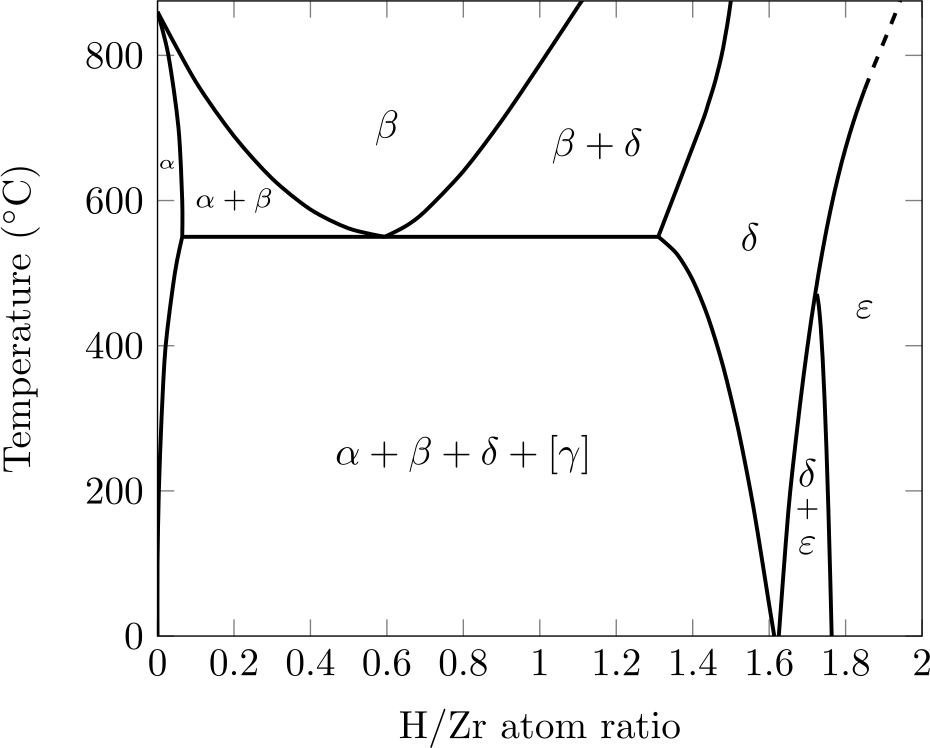
\includegraphics[height=2.50in,width=3.00in,viewport=0 0 930 748,clip]{Figures/Phase_diagram-Zr_H-systems.png}
\caption{\tiny \textrm{Phase diagram Zr-H systems.}}
\label{Fig:Phase_diagram-Zr_H-systems}
\end{figure}
\end{frame}

\begin{frame}
	\frametitle{研究内容}
	\begin{itemize}
	\item 氢化锆($\mathrm{ZrH}_{1.85-1.88}$)固体在高温(如$T=600^{\circ}\mathrm{C}$)密闭真空环境中,氢原子脱离氢化锆向外部空间中扩散的物理过程、扩散量及相应的扩散系数
	\item 氢化锆($\mathrm{ZrH}_{1.85-1.88}$)固体表面存在$\mathrm{ZrO}_2$涂层的条件下,氢原子脱离氢化锆向外部空间中扩散的物理过程、扩散量及相应的扩散系数
	\item 给定密闭空间体积,氢原子扩散后,整个扩散过程达到平衡时氢气的浓度
	\item 氢化锆($\mathrm{ZrH}_x$)固体中,不同浓度比例的氢(如$x=1.70$、$x=1.80$等)所对应的起始扩散温度
	\item 上述参数与表面$\mathrm{ZrO}_2$涂层的厚度的关系
	\end{itemize}
\end{frame}

\section{研究方法}
\begin{frame}
	\frametitle{研究方法}
研究的主要难点是获得锆及原子的势函数,势函数是分子动力学模拟的基础,包括
  \begin{columns}
	  \column{0.35\textwidth}
\begin{itemize}
	\item $\mathrm{Zr}$-$\mathrm{Zr}$的势函数
	\item $\mathrm{Zr}$-$\mathrm{H}$的势函数
	\item $\mathrm{Zr}$-$\mathrm{O}$的势函数
	\item $\mathrm{H}$-$\mathrm{O}$势函数
\end{itemize}
	  \column{0.70\textwidth}
\begin{figure}[!ht]
\centering
\vspace*{-0.05in}
\includegraphics[height=1.20in,width=2.30in,viewport=0 0 1316 735,clip]{Figures/Interstitial_sites-used-by-H-for-occupancy-in-hcp_Zr.png}
\caption{\tiny \textrm{Interstitial sites used by H for occupancy in HCP Zr.}}
\label{Fig:Interstitial_sites-used-by-H-for-occupancy-in-hcp_Zr}
\end{figure}
  \end{columns}
每一类势函数构造需要至少\textrm{150}个百原子($10^2$量级)的模型,通过\textrm{DFT}计算获得基态能量和原子受力,总的原子模型约$10^3$量级,每次并发模型计算任务约为\textrm{5$\sim$20},平均每个模型计算时间为1天,以当前的计算资源估计,预计至少三-四个月完成相关模型的计算任务
\end{frame}

\begin{frame}
	\frametitle{机器学习势函数的构建}
%	构建\textrm{nep}势函数($\mathrm{Zr}$-$\mathrm{H}$势、$\mathrm{Zr}$-$\mathrm{O}$势)的主要步骤
	\begin{itemize}
		\item 准备各类所需的计算模型,完成模型的体系基态能量和原子受力的\textcolor{magenta}{\textrm{DFT}计算}
%		\item 针对各模型,定义合适的\textcolor{blue}{描述符}:~与键长、键角和二面角相关
%			{\fontsize{6.2pt}{4.2pt}\selectfont{\begin{displaymath}
%				\begin{aligned}
%					G_i^2=&\sum_{j\neq i}\mathrm{e}^{-\eta(r_{ij}-r_s)^2}f_c(r_{ij})\\
%					G_i^3=&2^{1-\zeta}\sum_{j,k\neq i}(1+\lambda\cos\theta_{ijk})^{\zeta}\mathrm{e}^{-\eta(r_{ij}^2+r_{ik}^2+r_{jk}^2)}f_c(r_{ij})f_c(r_{ik})f_c(r_{jk})\\
%					G_i^9=&2^{1-\zeta}\sum_{j,k\neq i}(1+\lambda\cos\theta_{ijk})^{\zeta}\mathrm{e}^{-\eta(r_{ij}^2+r_{ik}^2)}f_c(r_{ij})f_c(r_{ik})
%				\end{aligned}
%			\end{displaymath}}}
		\item 选定模型中的一部分结构及其能量和原子受力,应用机器学习方法(神经网络),用来\textcolor{magenta}{训练机器学习势}
		\item \textcolor{magenta}{优化}训练集的\textcolor{blue}{描述符},进一步改善机器学习势
		\item \textcolor{magenta}{评估并测试}产生的机器学习势
	\end{itemize}
\end{frame}
	
%\begin{frame}
%	\frametitle{神经网络势的训练}
%	能量的表示
%	\begin{displaymath}
%		E_i=f_1^3\bigg\{b_1^3+\sum_{k=1}^{\mathrm{M}_{\mathrm{layer},2}}\omega_{n1}^{23}f_n^2\bigg[b_n^2+\sum_{m=1}^{\mathrm{M}_{\mathrm{layer},1}}\omega_{mn}^{12}f_m^1\bigg(b_m^1+\sum_{l=1}^{\mathrm{M}_{\mathrm{sym}}}\omega_{lm}^{01}G_{ij}\bigg)\bigg]\bigg\}
%	\end{displaymath}
%神经网络的优化函数
%\begin{displaymath}
%	\Gamma=\sum_{n=1}^{N_{\mathrm{struct}}}(E_{\mathrm{NN}}^n-E_{\mathrm{ref}}^n)^2+\beta^2\sum_{n=1}^{N_{\mathrm{struct}}}\sum_{m=1}^{3N_{\mathrm{atom}}^n}(F_{n,\mathrm{NN}}^m-F_{n,\mathrm{ref}}^m)^2
%\end{displaymath}
%\end{frame}
%
\begin{frame}
	\frametitle{计算任务进程:~\textrm{Zr-Zr}为例}
%	构造\textrm{Zr-Zr}相互作用势函数
	模型的来源与生产
	\begin{itemize}
		\item 由\textrm{Materials Project}选取一部分结构
		\item 通过\textrm{AIMD}模拟过程截取部分中间结构\textrm{(snapshots)}
	\end{itemize}
	计算模型的概况
	\begin{itemize}
		\item 模型类型:~\textrm{700$\sim$800}
		\item 每个模型:~约\textrm{120}原子
		\item 每个模型的\textrm{DFT}计算:~\textrm{64~cores}/\textrm{2.5~h}
	\end{itemize}
\end{frame}

\frame
{
	\frametitle{初始模型的来源}
{\fontsize{9.0pt}{7.2pt}\selectfont{
	\begin{enumerate}
		\item \textcolor{blue}{小胞扰动}:~包含单斜\textrm{hcp-Zr}、\textrm{\ch{ZrH}$_{1.5}$}、$\varepsilon$-\textrm{\ch{ZrH2}}、$\delta$-\textrm{\ch{ZrH2}}晶胞,对晶胞中所有原子随机施加微小位移,形成不同构型
		\item \textcolor{blue}{缩放和微扰}:~选取三种化学计量比\textrm{\ch{ZrH}$_{0.5}$}、\textrm{\ch{ZrH_{1.0}}}、\textrm{\ch{ZrH}}$_{1.5}$,创建超胞,缩放、微扰
		\item \textcolor{blue}{源自\textrm{Materials~Project}~结构}:~从\textrm{Materials~Project}%\footnote{MaterialsProject是知名的材料数据库,除MaterialsProject外,其他材料模拟的初始模型结构的来源的数据库还有
% https://oqmd.org/materials/entry/10100
% https://next-gen.materialsproject.org/materials?formula=Y
% http://crystalium.materialsvirtuallab.org/}
				下载约\textrm{20}个结构,对其进行原子坐标微扰
			\item \textcolor{blue}{表面结构}:~以$\delta$-\textrm{\ch{ZrH2}}为代表相,构建\{100\}、\{110\}、\{111\}等低指数表面,采样\textrm{\ch{ZrH}$_{0.5}$}、\textrm{\ch{ZrH}$_{1.0}$}、\textrm{\ch{ZrH}$_{1.5}$},对每种\textrm{slab}进行一次随机微扰
			\item \textcolor{blue}{空位、自间隙原子、氢原子在不同配位间隙(四面体/八面体)的结构}:\\
				构造\textrm{\ch{Zr}}、\textrm{\ch{ZrH}$_{0.5}$}、\textrm{\ch{ZrH}$_{1.0}$}、\textrm{\ch{ZrH}$_{1.5}$}、\textrm{\ch{ZrH}$_{2}$}的超晶胞,对其中的\textrm{Zr}配位结构缩放,复制结构并进行晶格和坐标微扰
\begin{figure}[!ht]
\centering
\vspace*{-0.05in}
\includegraphics[height=1.20in,width=2.30in,viewport=0 0 1316 735,clip]{~/Documents/Latex_Beamer/Figures/Interstitial_sites-used-by-H-for-occupancy-in-hcp_Zr.png}
\caption{\tiny \textrm{Interstitial sites used by H for occupancy in HCP Zr.}}
\label{Fig:Interstitial_sites-used-by-H-for-occupancy-in-hcp_Zr}
\end{figure}
			\item \textcolor{blue}{\textrm{NPT}系综采样}:~\textrm{\ch{Zr}}、\textrm{\ch{ZrH}$_{0.25}$}、\textrm{\ch{ZrH}$_{0.75}$}、\textrm{\ch{ZrH}$_{1.0}$}、\textrm{\ch{ZrH}$_{1.5}$}、\textrm{\ch{ZrH}$_{2}$}在不同的温度点运行\textrm{5~ns NPT~MD},每个温度点间隔抽取\textrm{5}个结构
			\item \textcolor{blue}{单轴、三轴拉伸与压缩}:~先进行\textrm{NPT}系综等温平衡,在\textrm{NVT}系综下以一定应变率进行单轴拉伸、压缩,并间隔抽取结构
		\end{enumerate}}}
}

%\subsection{氢化锆材料中的原子扩散}
\frame
{
	\frametitle{氢化锆材料中的原子扩散}
研究氢化锆中的原子扩散,重点考虑氢原子的扩散行为,特别是扩散行为受温度变化的影响
\begin{enumerate}
	\item 氢化锆(\textrm{\ch{ZrH}}$_{1.85-1.88}$)中氢原子由体相向外部空间中扩散的物理过程、扩散量及相应的扩散系数:\\
		{\fontsize{6.2pt}{4.2pt}\selectfont{通过氢化锆中氢原子经基本氢原子位置、填隙(四面体配位和八面体配位)空位、缺陷空位向体系表面的扩散行为描述,考虑\textrm{NVT}系综,得到氢原子在氢化锆体相的扩散系数;考虑氢原子结合形成氢气后,氢气分子在氢化锆中的动力学行为,计算氢分子在氢化锆体相的扩散系数}}
	\item 氢化锆(\textrm{\ch{ZrH}}$_{1.85-1.88}$)固体表面存在\textrm{\ch{ZrO2}}涂层的条件下,氢原子脱离氢化锆向外部空间中扩散的物理过程、扩散量及相应的扩散系数:\\
		{\fontsize{6.2pt}{4.2pt}\selectfont{通过氢原子穿越氢化锆-氧化锆界面、进入氧化锆涂层表面的动力学过程,以及在氧化锆涂层内与氧原子的扩散行为;考虑氢原子与氧原子的结合,在高温下形成水分子后的扩散,并计算扩散系数}}
	\item 给定密闭空间体积,氢原子扩散后,整个扩散过程达到平衡时氢气的浓度\\
		{\fontsize{6.2pt}{4.2pt}\selectfont{通过模拟氢化锆表面氢气吸附并形成氢原子并进入氢化锆体相,确定高温下,氢化锆与表面氢气表面平衡时的氢气分压估计,得到平衡太氢气的浓度}}
	\item 氢化锆(\textrm{\ch{ZrH}}$_x$)固体中,不同浓度比例的氢(如$x=1.70$、$x=1.80$等)所对应的起始扩散温度:\\
		{\fontsize{6.2pt}{4.2pt}\selectfont{根据\textrm{NVT}系综,结合氢气分压,确定不同氢比例下,氢分子扩散的起始温度,并用实验结果检验}}
	\item 上述参数与表面\textrm{\ch{ZrO2}}涂层的厚度的关系\\
		{\fontsize{6.2pt}{4.2pt}\selectfont{改变模型中表面涂层的厚度(\textrm{\ch{ZrO2}}层数),研究表面图层\textrm{\ch{ZrO2}}的影响}}
\end{enumerate}
}

%\subsection{氢化锆-氧化锆中可能存在的化学反应}
%\textcolor{red}{\hl{2025-03-04}}增补:~\hl{x-y-z}
\frame
{
	\frametitle{氢化锆-氧化锆中可能存在的化学反应}
工程和实验上,研究氢原子和氢气在氢化锆体相、氢化锆-氧化锆界面的扩散,每隔一定的时间,测定密闭气相的组分分压、分离气体测定色谱,确定其中\ch{H2}的含量。根据实现中在位分离的气体推测,可能的化学反应主要包括\\
{\centering
	\textrm{\ce{ZrH\textit{x} = Zr + $\frac{x}2$H2 ^}}\\
	\textrm{\ce{H2 (\textit{g}) + CO2 (\textit{g}) = CO (\textit{g}) + H2O}} \\
	\textrm{\ce{Zr + 2 CO2 (\textit{g}) = ZrO + 2 CO (\textit{g})}} \\
	\textrm{\ce{Zr + 2 CO2 (\textit{g}) = ZrC + ZrO2}}\\
}
应用理论模拟方法确定发生的化学反应,主要从反应热力学和动力学角度考虑:
\begin{enumerate}
	\item \textcolor{blue}{化学热力学}:\\
		{\fontsize{6.2pt}{4.2pt}\selectfont{主要借助\textrm{DFT}计算,确定在工作温度范围内$(400\sim700^{\circ}\mathrm{C})$各反应的反应自由能,初步确定可自发进行的化学反应。注意在上述反应中,考虑了固体中存在碳,使得反应更为复杂}}
	\item \textcolor{blue}{化学动力学}:\\
		{\fontsize{6.2pt}{4.2pt}\selectfont{根据热力学条件确定可能的动力学反应后,选用高精度的动力学力场,模拟若干原子(一般不超过10个原子,包括氢化锆、氢气、氧化锆、二氧化碳等)彼此接近和远离的可能组合,获得上述反应可能的动力学过程,确定各反应物-产物形成过程中形成的中间态结构,确定反应中的活化能和决速步,并通过第一原理分子动力学的\textrm{CI-NEB}方法检验反应动力学的可能性}}
\end{enumerate}
化学反应涉及化学键的形成与断裂,存在电子转移过程,特别是有关过渡态的模拟与推测,对计算精度的要求高,因此对原子间势函数和\textrm{DFT}能量计算的要求都比较高,即使应用机器学习势函数,整体的计算量仍将会相当可观
}

%\subsection{氢化锆的晶格振动声子}
\frame
{
	\frametitle{氢化锆的晶格振动声子}
应用机器学习势,可以比较精确地得到工作温度下,氢化锆的声子振动模式。因为氢原子在氢化锆体相扩散,将引起声子振动模式的变化,声子模式随温度和原子扩散的变化,可以确定工况温度下最优氢含量的范围。前述计算已经确定,当阻氢涂层氧化锆的存在,氢的扩散将会受到影响。而优化氢含量可以作为理论估算的阻氢表面涂层厚度的依据。将由声子振动优化得到的涂层厚度与前述计算得到的涂层厚度对比,检验两类计算的合理性
}

%\appendix
%%------------------------------------------------------------------------Reference----------------------------------------------------------------------------------------------
%		\frame[allowframebreaks]
%		{
%\begin{thebibliography}{99}
%\frametitle{主要参考文献}
%{\tiny
%%	\bibitem{PhysCN40-477_2011}曹则贤, \textit{Secular,equation}, \textit{物理}, \textbf{40} \textrm{(2011), 477}
%	\bibitem{PR136-B864_1964}\textrm{P. Hohenberg and W. Kohn, \textit{Phys. Rev.} \textbf{136} (1964), B864}
%	\bibitem{PR140-A1133_1965}\textrm{W. Kohn and L.J. Sham, \textit{Phys. Rev.} \textbf{140} (1965), A1133}
%	\bibitem{JPC12-4409_1979}\textrm{J. Ihm, A. Zunger and L. Cohen, {\textit{J. Phys. C}} \textbf{12} (1979), 4409}
%	\bibitem{PRB41-7892_1990}\textrm{D. Vanderbilt. \textit{Phys. Rev.} B, \textbf{41} (1990), 7892} 
%	\bibitem{JPCM6-8245_1994}\textrm{G. Kresse and J. Hafner. J. Phys: \textit{Condens. Matter}, \textbf{6} (1994), 8245}
%	\bibitem{PRB50-17953_1994}\textrm{P. E. Bl\"ochl. \textit{Phys. Rev.} B, \textbf{50} (1994), 17953}
%	\bibitem{PRB59-1758_1999}\textrm{G. Kresse and D. Joubert \textit{Phys. Rev.} B, \textbf{59} (1999), 1758}
%	\bibitem{PRB12-3060_1975}\textrm{O. K. Andersen. \textit{Phys. Rev.} B, \textbf{12} (1975), 3060}
%	\bibitem{JMP22-2433_1981}\textrm{M. Weiner. \textit{J. Math. Phys.}, \textbf{22} (1981), 2433}
%	\bibitem{PRB26-4571_1982}\textrm{M. Weinert, E. Wimmer and A. J. Freeman. \textit{Phys. Rev.} B, \textbf{26} (1982), 4571}
%	\bibitem{Andersen_Book}\textrm{O. K. Andersen. \textit{Computational Methods in Band Theory} (Plenum, New York, USA, 1971)}
%        \bibitem{Singh}\textrm{D. J. Singh. \textit{Plane Wave, PseudoPotential and the LAPW method} (Kluwer Academic, Boston,USA, 1994)}					%
%	\bibitem{Singh}\textrm{D. J. Singh. \textit{Plane Wave, PseudoPotential and the LAPW method} (Kluwer Academic, Boston,USA, 1994)}
%	\bibitem{Xie-Lu}谢希德、陆栋\:主编, {\textit{固体能带理论}}\:复旦大学出版社, 上海, 1998
%	\bibitem{Nemoshkalenko-Antonov}\textrm{V. V. Nemoshkalenko and V. N. Antonov. \textit{Computational Methods in Solid State Physics} (Gordon and Breach Science Publisher, Amsterdam, The Netherlands, 1998)}
%	\bibitem{Elect_Stru}\textrm{Richard. M. Martin. \textit{Electronic Structure: Basic Theory and Practical Methods} (Cambridge University Press, Cambridge, England, 2004)}
%	\bibitem{Xu_Li_Wang}徐光宪、黎乐民、王德民, {\textit{量子化学——基本原理和从头计算法}}\;\textrm{({\textit{上、中}})}\:科学出版社, 北京, 1980
%%	\bibitem{SSC114-15_2000}\textrm{E. Sj\"ostedt, L. Nordstr\"om and D. J. Singh. \textit{Solid State Commun.}, \textbf{114} (2000), 15}
%}
%\end{thebibliography}
%\nocite*{}
%}
